%%=============================================================================
%% Methodologie
%%=============================================================================

\chapter{Methodologie}
\label{ch:methodologie}

%% TODO: Hoe ben je te werk gegaan? Verdeel je onderzoek in grote fasen, en
%% licht in elke fase toe welke stappen je gevolgd hebt. Verantwoord waarom je
%% op deze manier te werk gegaan bent. Je moet kunnen aantonen dat je de best
%% mogelijke manier toegepast hebt om een antwoord te vinden op de
%% onderzoeksvraag.

\section{Literatuurstudie Android Wear}
\label{sec:androidwear}
Android Wear is Google's platform voor wearables. Een wearable wordt beschreven als een computer of geavanceerd elektronisch toestel dat geïncorporeerd is in een accessoire gedragen op het lichaam of in een kledingstuk. \autocite{Dictionary}
We lijsten enkele van de  belangrijkste kenmerken van Android Wear op. \autocite{Techradar}.
Android Wear is gebouwd voor kleinere toestellen en met hands-free gebruik in het achterhoofd. Het maakt de toegang tot enkele van uw smartphone's makkelijkste functionaliteiten zo makkelijk als kijken naar uw pols. Het is vooral bedoeld om de notificaties van uw smartphone makkelijk te weergeven zodat niet elke keer gezocht moet worden naar de smartphone in de broekzak. Gebaseerd op uw Google zoekopdrachten zullen real-time scores van uw favoriete sportteam, verkeerscondities of afspraken in uw agenda weergeven worden. Als het Android Wear toestel NFC (Near Field Communication) ingebouwd heeft, kan er in verschillende landen (momenteel Australië, Hong Kong, Ierland, Japan, Nieuw-Zeeland, Polen, Singapore, Verenigd Koninkrijk en de Verenigde Staten) ook met de wearable betaald worden via Android Pay. \autocite{Androidpay} Ook spraakherkenning kon niet ontbreken in de Android Software. Door deze technologie kan je de op de wearable spraakherkenning activeren door "Okay, Google" te zeggen of door de aanknop ingedrukt te houden. Google Assistant zal u hierop verderhelpen. Android Wear is compatibel met smartphones die werken op Android 4.3 en hoger of iOS 9 en hoger. Eén van de belangrijkste app-categorieën op Android Wear zijn de gezondheidsapps. Hiervoor wordt standaard gebruik gemaakt van Google Fit. Met Google Fit kan je kiezen tussen verschillende workouts tijdens het sporten, of bijvoorbeeld een dagelijks doel instellen voor het aantal stappen dat u wil nemen.  
\begin{figure}[H]
	\centering
	\caption{\textit{Enkele voorbeelden van smartwatches gebruikmakend van Android Wear}}
	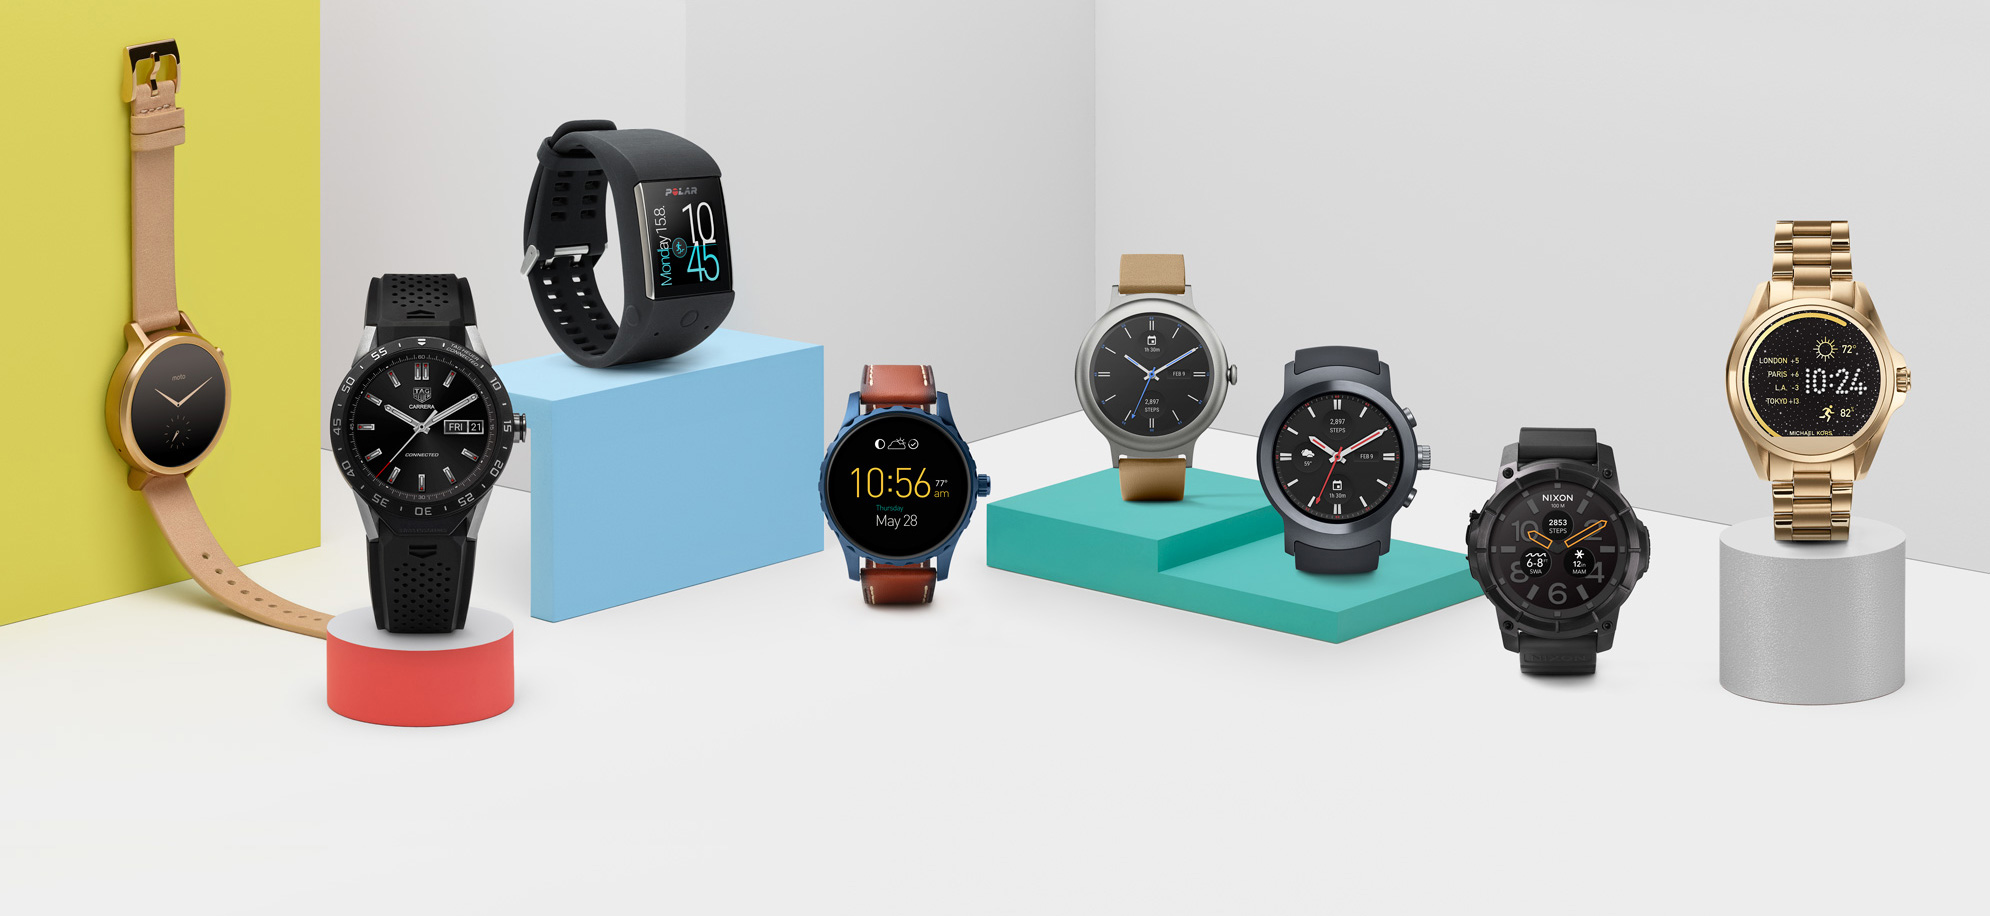
\includegraphics[width=10cm, height=10cm, keepaspectratio]{img/WearExamples}\\[.5cm]
\end{figure}
%% TODO:
%% Uit je probleemstelling moet duidelijk zijn dat je onderzoek een meerwaarde
%% heeft voor een concrete doelgroep (bv. een bedrijf).
%%
%% Wees zo concreet mogelijk bij het formuleren van je
%% onderzoeksvra(a)g(en). Een onderzoeksvraag is trouwens iets waar nog
%% niemand op dit moment een antwoord heeft (voor zover je kan nagaan).
\subsection{Wat is een APK en uit wat bestaat dit?}
APK staat voor Android Application Package. Een APK is een applicatiebestand klaar voor installatie op een Android-toestel. Het gecompresseerde APK bestand, een ZIP archief in JAR-formaat, wordt gedistribueerd naar Android gebruikers voor de installatie op hun smartphone, tablet of wearable. \autocite{PCMag}
Een APK bestand bestaat normaliter uit volgende elementen : 
\subsubsection{Elementen APK}
\begin{enumerate}
	\setlength\itemsep{2em}
	\item \textbf{classes.dex} \newline
	Bevat gecompileerde applicatiecode, getransformeerd naar een DEX bytecode. Het is mogelijk dat er meerdere DEX bestanden in de APK staan als er multidex gebruikt wordt om de 65536 limiet te overkomen. Vanaf Android 5.0, met de introductie van ART runtime, worden deze bestanden gecompileerd naar OAT bestanden door de compiler bij de installatie en worden deze op de data partitie van het toestel geplaatst. 
	\item \textbf{res/} \newline
	Deze folder bevat de meeste XML-bestanden en drawables (bijvoorbeeld PNG- of JPEG-bestanden) in mappen met verschillende kwalificaties, zoals -mdpi en -hdpi voor schermdichtheden, -sw600dp of -large voor schermgroottes, en -en, -de, -pl voor talen. De XML bestanden worden automatisch gecompileerd naar een compactere binaire representatie, dus deze kunnen niet met een teksteditor geopend worden vanuit de APK. 
	\item \textbf{resources.arsc}\newline
	Sommige resources en identifiers worden gecompileerd naar dit bestand. Het wordt normaal ongecomprimeerd opgeslagen in de APK voor snellere toegang tijdens runtime. Dit bestand manueel comprimeren kan een makkelijke oplossing lijken, maar dit is geen goed idee door 2 redenen: Eén, Play Store comprimeert alle data voor transfer automatisch en twee, dit bestand comprimeren in de APK verspilt systeem resources (RAM) en performantie (vooral de opstarttijd van de app).
	\item \textbf{AndroidManifest.xml}\newline
	Gelijklopend met andere XML resources wordt de applicatie Manifest getransformeerd naar een binair formaat tijdens de compilatie. De Play Store gebruikt bepaalde informatie in de AndroidManifest om te bepalen of een APK kan geïnstalleerd worden op een bepaald toestel. Zo zijn er controles op toegelaten schermdichtheden of schermgroottes, beschikbare hardware en kenmerken (bijvoorbeeld aanwezigheid van een touchscreen). De inhoud van het Manifest kan geïnspecteerd worden na compilatie. Gebruik hiervoor de aapt tool van de Android SDK: 
	\lstset{aboveskip=10pt, belowskip=0pt}
	\begin{lstlisting}[backgroundcolor = \color{lightgray}, xleftmargin = 2cm,
	framexleftmargin = 1em]
	$ aapt dump badging your_app.apk
	\end{lstlisting}
	\item \textbf{libs/}\newline
	Alle native libraries (*.so bestanden) zullen in submappen geplaatst worden genaamd naar de ABI (CPU architectuur, bv. x86, \texttt{x86\_64}, armeabi-v7a) die ze als doel hebben onder de libs/ map. Normaal worden deze uit de APK gekopieerd naar de datapartitie tijdens het installeren van de applicatie. Echter, sinds de APK zelf nooit aangepast wordt zolang deze op het toestel van de gebruiker staat, neemt dit dubbel zoveel plaats in voor elke native library. 
	\item \textbf{assets/}\newline
	Deze map zal gebruikt worden voor alle bestandsonderdelen die niet als Android-type resources gebruikt zullen worden. Meestal zullen dit lettertypebestanden of game data zijn, zoals levels of textures, samen met andere applicatiedata die direct geopend moet kunnen worden als een file stream.
	\item \textbf{META-INF/}\newline
	Deze map is aanwezig in ondertekende APKs en bevat een lijst van alle bestanden in de APK met hun handtekening. Momenteel werkt het ondertekenen van bestanden in Android door het verifiëren van de handtekening tegen de ongecomprimeerde bestandsinhoud van het archief, één voor één. Dit heeft enkele interessante gevolgen. Doordat elke onderdeel van een ZIP bestand apart opgeslagen wordt, betekent dit dat je individuele bestanden hun compressieniveau kan aanpassen zonder ze opnieuw te ondertekenen. De verificatie van de handtekening zal echter falen wanneer een bestand verwijderd wordt uit het archief nadat het ondertekend werd. 
\end{enumerate}

\begin{figure}[H]
	\centering
	\caption{\textit{De structuur van de APK}}
	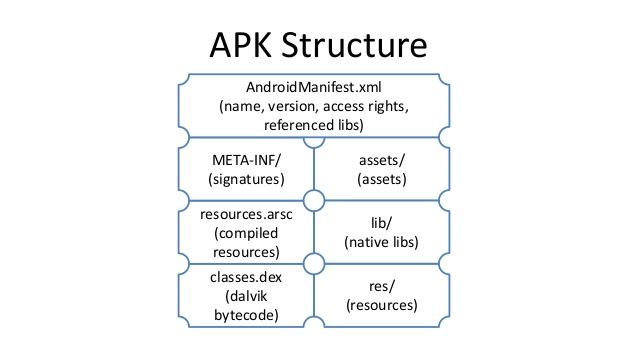
\includegraphics[width=10cm, height=10cm, keepaspectratio]{img/ApkStructure}\\[.5cm]
	
\end{figure}
\subsection{Conclusie APK-structuur}
Een APK bestaat dus uit 7 onderdelen. Deze onderdelen zullen echter wel verschillen van grootte. Indien de app veel afbeeldingen bevat zal de map res/ het grootste deel van de APK-grootte innemen. Indien de app veel code bevat zal het classes.dex bestand groter worden. In de proof-of-concept app, die later in deze studie wordt toegelicht, konden we volgende verhoudingen waarnemen tussen de groottes van de verschillende onderdelen: 
\begin{enumerate}
	\item classes.dex: 0.4\%
	\item res/: 98.3\%
	\item resources.arsc: 1.1\%
	\item AndroidManifest.xml: kleiner dan 0.01\%
	\item libs/: kleiner dan 0.01\%
	\item assets/: kleiner dan 0.01\%
	\item META-INF/: 0.2\% 
\end{enumerate}

\subsection{Verschillende app-profielen Android Wear}
Verder in deze studie zullen de verschillende compressietechnieken toegepast worden op een proof-of-concept app binnen elk van de 3 profielen (foto-apps, fitness-apps, CPU-intensieve apps). Hierdoor kan binnen elk app-profiel gekeken worden welke technieken het meeste invloed zullen hebben op de grootte van de APK. Ook zal voor elk app-profiel onderzocht worden of er al dan niet negatieve bijwerkingen zijn voor de prestaties van de app na compressie en hoe groot deze bijwerkingen zijn. Op deze manier kan dit onderzoek voor de ontwikkelaars van elk type app nagaan welke technieken voor hun app in ontwikkeling het meest effect zullen hebben op de grootte van de APK. Aan de hand van de resultaten van het onderzoek kan dan ook de afweging gemaakt worden of er voor hun applicatie niet te veel moet ingeboet worden op vlak van CPU- en geheugenprestaties van de app.
\subsubsection{Fitness-apps}
Deze apps zullen de gebruiker vooral helpen bij het opvolgen van lichamelijke inspanningen en opvolging van voeding. Bij deze apps wordt meestal gebruikgemaakt van de ingebouwde GPS in het Android Wear toestel. Doordat deze GPS constant actief is, zal het batterijgebruik van deze apps zeer hoog liggen.
\subsubsection{Foto-apps}
Apps die veel gebruikmaken van foto's zullen in het algemeen vrij veel opslagruimte in beslag nemen, aangezien elke foto in de app meegeleverd wordt en de grootte van een foto snel kan oplopen tot 1MB. Indien de foto's niet meegeleverd worden in de APK van de app, dienen de foto's gedownload te worden van het internet en zal er dus meer netwerkactiviteit gebruikt worden en CPU verbruik om de foto te genereren op de juiste plaats in de app.
\subsubsection{CPU-intensieve apps}
Apps die veel (visuele) informatie moeten genereren tijdens runtime, zullen in het algemeen een hoog CPU verbruik hebben. Een voorbeeld hiervan is een app die muziek afspeelt en intussen visuele effecten afbeeldt die gegenereerd worden op het tempo van de afgespeelde muziek.  

\section{Verschillende compressietechnieken}
\label{sec:compressietechnieken}

Uit de richtlijnen van Google voor het verkleinen van de grootte van de APK werden volgende technieken gekozen om te onderzoeken \autocite{googlereduceapksize}: 

\subsubsection{Gebruik Proguard en Dexguard}
Uit een interview met Cozmos, het bedrijf waarbij mijn co-promotor Joris Missiaen werkzaam is blijkt dat zij deze tools ook gebruiken : 
\begin{quote}
	\colorbox{lightgray}{\parbox{350px}{"De belangrijkste tool om de grootte van een APK te beperken is Proguard. Proguard zorgt er niet enkel voor dat je code moeilijker leesbaar wordt bij reverse engineering maar het verwijdert ook al je ongebruikte code en resources.
			Bij de grotere klanten waar ook security van groot belang is maken we gebruik van Dexguard. Dexguard is de commerciële variant van Proguard en gaat een stap verder met zijn compressietechnieken maar biedt daarnaast ook tal van andere features aan."
	}}
\end{quote}
Deze andere features zijn dan bijvoorbeeld bescherming tegen static analysis, beveiliging tegen klonen van de APK/SDK en bescherming tegen piraterij. Ook beschermt Dexguard tegen dynamic analysis (APK beveiligen tijdens runtime) door omgeving- en certificaatcontroles. 

\subsubsection{Verwijder ongebruikte resources}
\label{sec:removeunusedresources}
De ingebouwde lint tool in Android Studio, een statische code analyzer, detecteert resources in de res/ map die in de code niet gerefereerd worden. Android Studio zal hiervan een melding maken, maar zal deze niet automatisch verwijderen. Libraries die u toevoegt kunnen ongebruikte resources meebrengen. Gradle kan deze automatisch verwijderen als ``shrinkResources`` in de build.gradle wordt toegevoegd. 

\subsubsection{Verklein resource gebruik van libraries}
\label{sec:minimizeresourceslibraries}
Wanneer u een Android app ontwikkelt, worden vaak externe libraries gebruikt om de gebruiksvriendelijkheid te verhogen. Deze libraries bevatten vaak elementen die voor desktops of servers bedoeld zijn, deze elementen kunnen uit de libraries verwijderd worden indien de licentie dit toestaat. Deze techniek wordt ook gebruikt door Cozmos volgens Joris Missiaen: 
\begin{quote}
	\vspace{-15ex}
	\colorbox{lightgray}{\parbox{350px}{"Bij het gebruik van libraries kan het handig zijn om enkel de modules in je project te importeren die je ook daadwerkelijk nodig hebt. Ook kan het nuttig zijn om verschillende libraries tegenover elkaar af te wegen en te kijken welke de laagste method count hebben, het best met het geheugen omgaan, het minste plaats innemen, enz. Stel dat je een library aan je project zou willen toevoegen om images in te laden dan zou je de afweging kunnen maken tussen Glide en Picasso. Picasso is bijvoorbeeld 3,5 keer kleiner dan Glide, maar anderzijds gebruikt Glide een pak minder geheugen om een image weer te geven. Dat zijn afwegingen die je moet maken."}}
	\vspace{-3ex}
\end{quote}

\subsubsection{Ondersteun enkele specifieke schermdichtheden }
\label{sec:supportspecificdensities}
Vanaf Android 4.4 worden verschillende schermdichtheden ondersteund (ldpi, mdpi, tvdpi, hdpi, xhdpi, xxhdpi en xxxhdpi). Het is niet nodig om elke afbeelding te exporteren naar elke dichtheid. Android zal automatisch de afbeelding schalen naar andere schermdichtheden als er geen specifieke export voorzien is. 

\subsubsection{Verminder animatieframes }
\label{sec:reduceanimationframes}
Voor elke frame in een animatie wordt een aparte afbeelding opgeslagen. Als er bijvoorbeeld een animatie aanwezig is met 30 FPS (frames per second) zullen er 30 afbeeldingen opgeslagen worden, maar vaak is bijvoorbeeld 15 FPS meer dan voldoende. Op deze manier zijn er dus maar half zoveel animatieframes nodig.
\begin{figure}[H]
	\centering
	\caption{\textit{Door vermindering FPS zullen minder aparte afbeeldingen per animatie opgeslagen worden}\newline}
	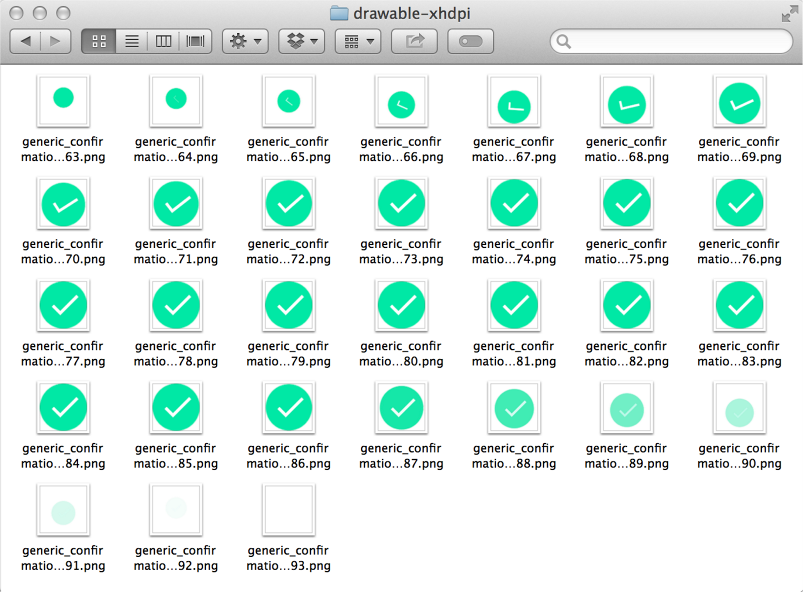
\includegraphics[width=10cm, height=10cm, keepaspectratio]{img/animation-frames}\\[.5cm]
	
\end{figure}
\subsubsection{Hergebruik resources }
\label{sec:reuseresources}
Het is mogelijk om voor elke variatie op een afbeelding (getint, met schaduw of geroteerd) een aparte resource op te slaan. Google raadt echter aan om één afbeelding te voorzien, en deze dynamisch tijdens runtime aan te passen. 
Android voorziet verschillende hulpprogramma's om de kleur van een afbeelding aan te passen.
\subsubsection{Comprimeer afbeeldingen }
\label{sec:compressimages}
De \cite{aapt} tool kan de afbeelding resources in res/drawable/ optimaliseren met lossless compressie. De tool kan bijvoorbeeld een true-color PNG bestand dat niet meer dan 256 kleuren bevat omzetten naar een 8-bit PNG met een kleurenpallet. Dit resulteert in een afbeelding van eenzelfde kwaliteit maar met een kleinere geheugenvoetafdruk. Deze tool kan geen PNG-bestanden in de asset/ folder verkleinen. Deze techniek wordt ook bij Cozmos gebruikt volgens Joris Missiaen: 
\begin{quote}
	\colorbox{lightgray}{\parbox{350px}{"Je kan al ruimte besparen door een juiste keuze te maken tussen JPG/PNG en verdere compressie toe te passen. Soms is ook geen volledige image nodig maar kan je opteren voor een 9-patch image of om een drawable in XML te definieren."}}
\end{quote}

\subsubsection{Gebruik WebP bestandformaat }
\label{sec:webp}
In plaats van PNG- of JPEG-bestanden, kan er ook gebruik gemaakt worden van het WebP formaat voor afbeeldingen. Dit formaat voorziet lossless compressie (zoals JPEG) en transparantie (zoals PNG) maar voorziet betere compressie dan beide andere formaten. Het gebruik van WebP heeft echter ook enkele nadelen. WebP-ondersteuning is niet beschikbaar bij versies lager dan Android 3.2 (API level 13). Het neemt ook een langere tijd voor het systeem om WebP bestanden te decoderen dan PNG bestanden. Bestaande BPM, JPG, PNG of statische GIF afbeeldingen kunnen naar het WebP formaat omgezet worden door Android Studio. 

\subsubsection{Gebruik vector graphics }
\label{sec:vectorgraphics}
Vector graphics kunnen gebruikt worden om resolutie-onafhankelijke iconen of andere schaalbare media te creëren. Deze afbeeldingen worden in Android gerepresenteerd als VectorDrawable objecten. Met een VectorDrawable object kan een 100-byte bestand een scherpe afbeeldingen genereren op de grootte van het scherm. 
Echter, het neemt een significante tijd voor het systeem om elk VectorDrawable object te genereren. Grote afbeeldingen kunnen zelfs nog meer tijd in beslag nemen om op het scherm te verschijnen. Daarom wordt aangeraden de VectorDrawable objecten enkel voor kleine afbeeldingen te gebruiken. 
\subsection{Verminder gebruik code}
\label{sec:reducecode}

\subsubsection{Verwijder automatisch gegenereerde code}
\label{sec:reducegeneratedcode}
Zorg dat u verstaat wat elke lijn gegenereerde code inhoudt en wat de voetafdruk ervan is. Zo zullen veel protocol buffer tools een groot aantal methodes en klassen genereren, die de grootte van de app kunnen verdubbelen of verdriedubbelen.

\subsubsection*{Verwijder enumeraties}
\label{sec:removeenumerations}
Elke enum kan 1 tot 1.4 KB grootte toevoegen aan uw app's classes.dex bestand. Deze toevoegingen kunnen snel oplopen voor complexe systemen of gedeelde libraries. Indien mogelijk gebruikt u best de @IntDef annotatie en ProGuard om enumeraties te strippen en om te zetten in integers. Deze conversie behoudt alle voordelen van enums. 
\subsubsection*{Verklein grootte native binaries}
\label{sec:reducesizenativebinaries}
Bij het gebruik van native code en de Android NDK (Native Development Kit, hierdoor kan je bepaalde delen van je app implementeren in native-code talen zoals C of C++) kan je de grootte van de app verkleinen door het optimaliseren van de code. Hiervoor zijn 2 technieken bruikbaar :
\begin{enumerate}
	\item \textbf{Debug symbolen verwijderen} \newline
	Wanneer de app niet meer in development is, zijn debug symbolen overbodig. Deze kan je uit de applicatie verwijderen door de ``arm-eabi-strip`` tool te gebruiken, deze zit ingebouwd  in Android NDK.
	\item \textbf{Vermijd het extraheren van native libraries} \newline
	Bewaar .so bestanden ongecompresseerd in de APK, en stel de ``android:extractNativeLibs`` vlag op false in het ``<application>`` element van je app manifest. Dit zal vermijden dat de PackageManager de .so bestanden uit de APK naar het bestandssysteem zal kopiëren tijdens de installatie, en zal als bijkomend voordeel hebben dat delta updates van de app kleiner zullen zijn. 
\end{enumerate}

\subsection{Voorzie meerdere APK's}
\label{sec:multipleapks}
De app kan inhoud bevatten die gebruikers downloaden maar nooit gebruiken, zoals regio- of taalgerelateerde informatie. Om een minimale download voor de gebruikers te voorzien, kan de app gesegmenteerd worden in verschillende APKs, gedifferentieerd door factoren zoals schermgrootte of GPU structuur.
Wanneer gebruikers de app downloaden zal hun toestel de correcte APK ontvangen gebaseerd op het toestel zijn instellingen en kenmerken. Op deze manier ontvangen hun toestellen geen inhoud bedoeld voor opties die het toestel niet heeft.


\section{Verband tussen compressie en prestaties apps}
\label{sec:verbandcompressieprestaties}
Bij Cozmos werd het volgende opgemerkt als verband tussen compressie en de prestaties van de apps :
\begin{quote}
	\colorbox{lightgray}{\parbox{350px}{"Er wordt zeker naar gekeken dat de performantie van de app goed zit. Bij het uitvoeren van network calls moet alles zo compact mogelijk zijn zodat een gebruiker ook onder een slechte verbinding kan blijven werken. Bij het tonen van meerdere afbeeldingen is het memory management zeer belangrijk om o.a. out of memory exceptions te vermijden. Op welk vlak de performantie een invloed heeft hangt af van ieder geval op zich. Je kan stellen dat er op één of meerdere van volgende punten verbetering merkbaar is": \begin{enumerate}
				\item \textbf{Grootte beperken}
				\item \textbf{Geheugen gebruik beperken}
				\item \textbf{Sneller laden}
			\end{enumerate}
	}}
\end{quote}


\section{Creatie proof-of-concept foto-app}
\label{sec:proofofconcept}

Om het onderzoek te onderbouwen, werd een Android Wear proof-of-concept app gecreëerd. Dit is een algemene applicatie, waarin verschillende elementen toegevoegd worden zoals media-bestanden en veel code. Het doel van de creatie van deze app is om de verschillende compressietechnieken hierop toe te passen en de resultaten grafisch voor te stellen. De applicatie draait op Android Wear 2.0. Deze versie werd op 09/02/2017 uitgebracht door Google.\autocite{Google} Doordat voor deze versie gekozen werd, kan de app als standalone app gebruikt worden. Dit houdt in dat de app op een smartwatch kan gebruikt worden onafhankelijk van een smartphone. De gebruikers kunnen meer taken, zoals muziek afspelen of foto's bekijken, op hun smartwatch uitvoeren zonder toegang tot een Android of iOS smartphone. De app zal als functie hebben om foto's weer te geven op de smartwatch, waar de gebruiker tussen kan wisselen door te tikken op het scherm. Op deze afbeeldingen werd vooraf nog geen compressie toegepast er werden afbeeldingen van een standaardgrootte gebruikt die dan automatisch geschaald werden naar de grootte van de image views. In de app zit ook een splashscreen verwerkt (scherm dat weergeven wordt tijdens het opstarten van de applicatie). 
\begin{figure}[H]
	\centering
	\caption{\textit{Hoofdscherm foto-app}}
	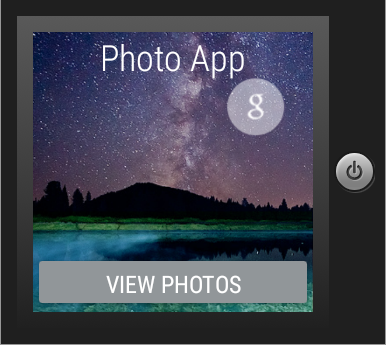
\includegraphics[width=7cm, height=7cm, keepaspectratio]{img/photoappmain}\\[.5cm]
\end{figure}
\begin{figure}[H]
	\centering
	\caption{\textit{Foto view}}
	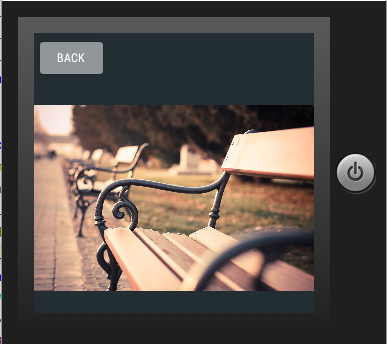
\includegraphics[width=7cm, height=7cm, keepaspectratio]{img/photoappgallery}\\[.5cm]
	
\end{figure}

\section{Verschillende technieken toepassen op proof-of-concept app}
\label{sec:techniekentoepassen}


\section{Prestaties en grootte app testen na toepassen technieken}
\label{sec:prestatiesgrootteapp}

\section{Testen van app door framework Brian Pinsard}
\label{sec:apptesting}